\section{Benutzerinteraktion}
\paragraph{Routed Events}
\begin{itemize}
    \item Interessante UI Ereignisse, auf die reagieren soll (Mouse, Keyboard oder Touch-Ereignisse)
    \item Routed Events können mit \code{Handled = "True"} unterbrochen/abgebrochen werden
    \item 2 Phasen: abwärts (Preview/Tunnelling) und dann aufwärts (Bubbeling) gerouted (wie bei HTML 5) 
    \item Preview Event wird vor dem eigentlichen Event ausgeführt (hier kann man prüfen, ob z.B die gedrückte Taste eine Nummer war)
\end{itemize}
% 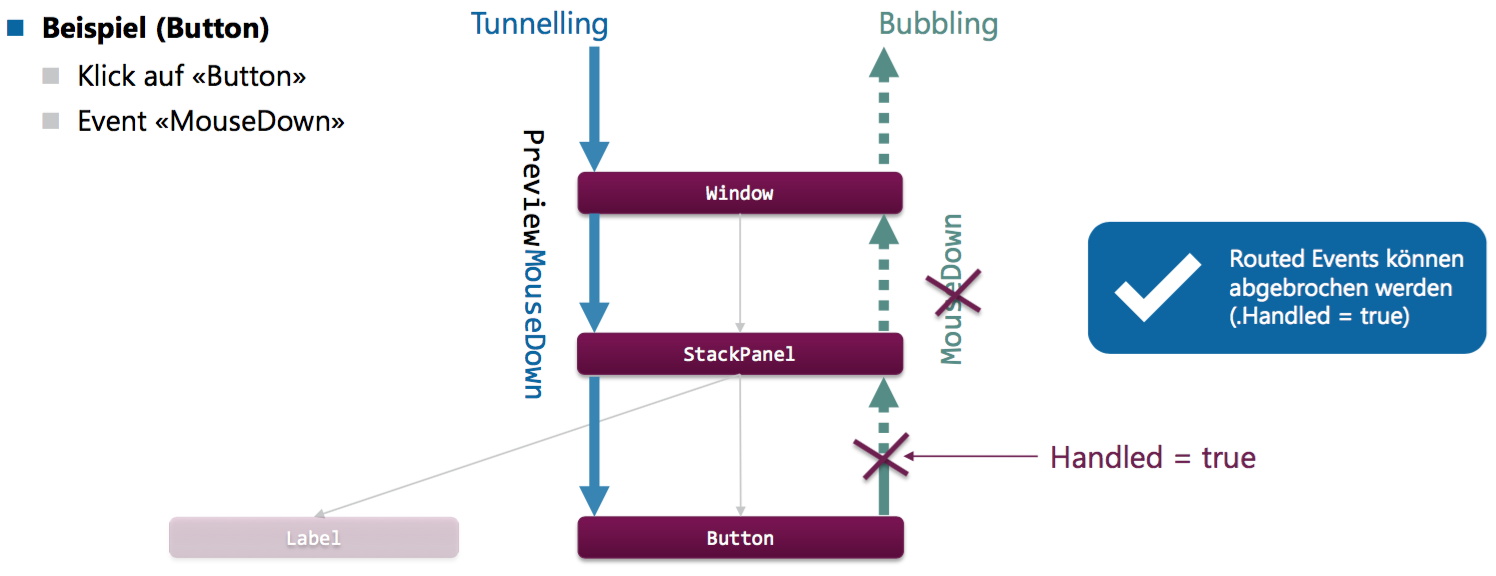
\includegraphics[scale=0.25]{RoutedEvent1.png}
% 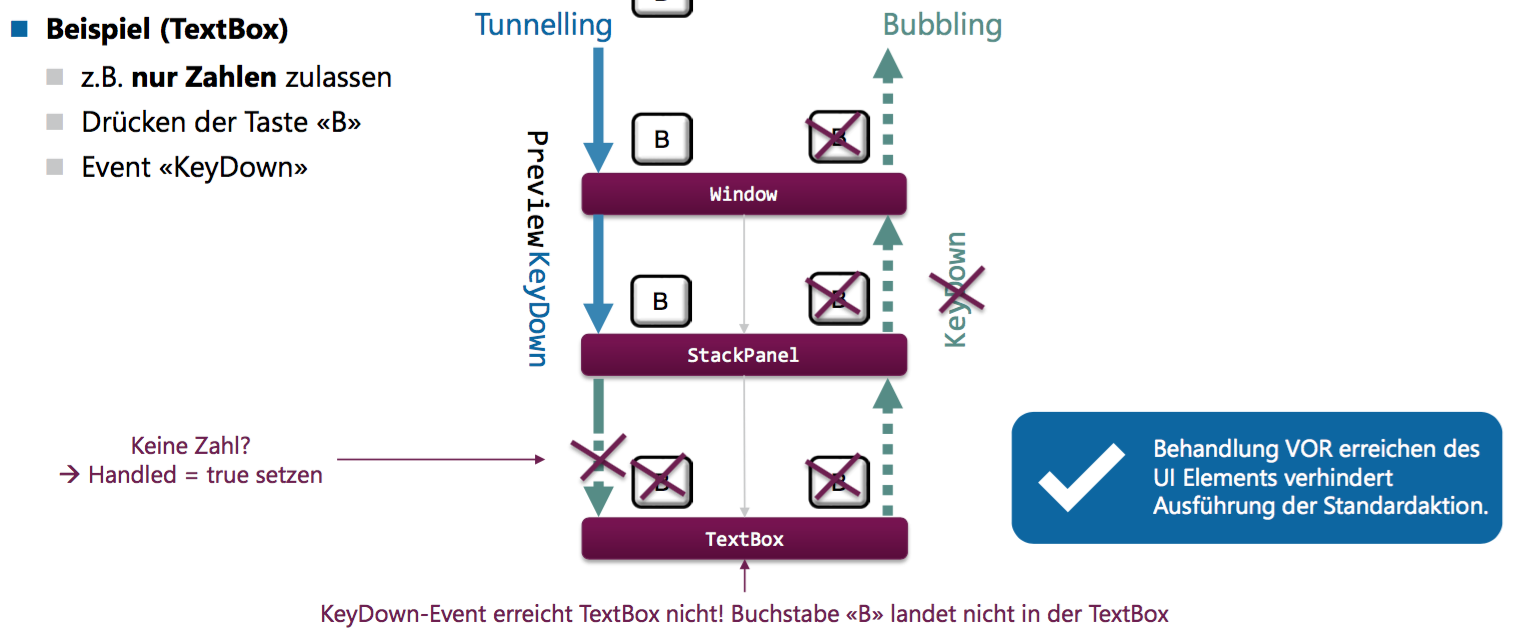
\includegraphics[scale=0.25]{RoutedEvent2.png}
UI Events können beim Ui Element selbst behandelt werden:
\begin{lstlisting}[language=xml]
<Button Name="SaveButton"
    PreviewMouseDown="SaveButton_OnPreviewMouseDown"
    MouseDown="SaveButton_OnMouseDown">Save</Button>
\end{lstlisting}


Oder beim Parent Element
\begin{lstlisting}[language=xml]
<StackPanel PreviewMouseDown="StackPanel_OnPreviewMouseDown">
    ...
    <Button Name="SaveButton"
        PreviewMouseDown="SaveButton_OnPreviewMouseDown"
        MouseDown="SaveButton_OnMouseDown">Save</Button>
    ...
</StackPanel>
\end{lstlisting}


Eine andere Alternative wäre mit Attached Events.
\begin{lstlisting}[language=xml]
<StackPanel Button.Click="StackPanel_OnClick">
    ...
    <Button Name="SaveButton" Click="SaveButton_OnClick">Save</Button>
    ...
</StackPanel>
\end{lstlisting}

Routed Events behandeln im Code Behind: \\
Grundlegend wenn UI Control einen Namen hat (Zugriff wie gewohnt)
\begin{lstlisting}
private void SaveButton_OnPreviewMouseDown(object sender, MouseButtonEventArgs e) { 
// Dinge prüfen, bevor das Event das Element erreicht hat } 
private void SaveButton_OnMouseDown(object sender, MouseButtonEventArgs e) { //Event behandeln } 
\end{lstlisting}
Geht auch wenn das UI Control keinen Namen hat (UI Control einen Namen geben und casten):
\begin{lstlisting}
private void SaveButton_OnMouseDown(object sender, MouseButtonEventArgs e) { 
var saveButton = sender as Button; }
\end{lstlisting}

\textbf{Beliebte Mouse Events:}
\begin{tabular}{ll}
MouseDown & MouseEnter* \\
MouseLeave* & MouseLeftButtonDown \\
MouseLeftButtonUp & MouseMove \\
MouseRightButtonDown & MouseRightButtonUp \\
MouseUp & MouseWheel
\end{tabular}

\textbf{Interessante Keyboard Events:} \\
\begin{tabular}{ll}
KeyDown & KeyUp \\
TextInput & 
\end{tabular}

\textbf{Interessante Touch-Events:} \\
\begin{tabular}{ll}
TouchDown & TouchEnter* \\
TouchLeave* & TouchMove \\
TouchUp & 
\end{tabular}
\\
* \textit{haben kein Preview Event}


\paragraph{RoutedEventArgs} RoutedEventArgs leiten von EventArgs ab. 
\begin{description}
\item[\code{Handled}] Boolean der aussagt, ob das Event behandelt wurde
\item[\code{OriginalSource}] Quell-Element (Hit-Testing) welches das Event ausgelöst hat
\item[\code{RoutedEvent}] Das RoutedEvent, welches mit diesem Objekt verknüpft ist
\item[\code{Source}] Element, welches das Event rapportiert hat
\end{description}

Die OriginalSource kann ein Kind-Element des Source-Elements sein, das per Hit-Testing als 1. Adressat des Events bestimmt wurde. Die Source ist das Element im Logical Tree, welches das Event rapportiert hat. Beispielsweise beim Subscribe auf MouseDown auf einem Button, wird das Event vom Button rapportiert (Source), wurde aber eigentlich vom Rahmen ausgelöst (OriginalSource).

\paragraph{Ableitende Klasse von RoutedEventArgs} Es gibt für verschiedene Input-Geräte Ableitungen von RoutedEventArgs. Auswahl von \verb+MouseEventArgs+:
\begin{itemize}
\item \textbf{LeftButton}: Zustand der linken Maustaste (Pressed/Released)
\item \textbf{MiddleButton}
\item \textbf{RightButton}
\item \textbf{Delta}: Mausradbewegung (-120/120)
\end{itemize}
Auswahl von \verb+KeyEventArgs+:
\begin{itemize}
\item \textbf{Key}: Taste (Enum)
\item \textbf{IsDown}
\item \textbf{IsUp}
\item \textbf{IsRepeat}
\item \textbf{SystemKey}: Die zusätzliche Taste, falls ALT-Taste gedrückt wurde. Key steht in \verb+Key.System+
\end{itemize}
\subsection{Drag \& Drop}
Drag \& Drop besteht aus 3 Phasen:
\begin{enumerate}
\item \textbf{Maustaste wird gedrückt:} Nach überschreiten einer Mindestdistanz wird die Aktion gestartet
\item \textbf{Während des Ziehens:} Steuerelemente unterhalb des Zeigers müssen melden, ob sie als Ziel infrage kommen
\item \textbf{Fallenlassen:} Steuerelement unterhalb des Mauszeigers muss eine Aktion mit dem bewegten Objekt durchführen
\end{enumerate}
Beispiel:
\begin{lstlisting}
public ObservableCollection<UserInfo> AvailableUsers { get; set; }
public ObservableCollection<UserInfo> SelectedUsers { get; set; }
public MainWindow()
{
    // Listen initialisieren und fuellen
    InitializeComponent();
    DataContext = this;
}
\end{lstlisting}
\paragraph{Phase 1} Maustaste wird gedrückt
\begin{lstlisting}[language=xml]
<ListBox Name="AvailableListBox" ItemsSource="{Binding AvailableUsers}"
    ItemTemplate="{StaticResource UserInfoTemplate}"
    PreviewMouseLeftButtonDown="AvailableListBox_ OnPreviewMouseLeftButtonDown"
    PreviewMouseLeftButtonUp="AvailableListBox_ OnPreviewMouseLeftButtonUp"
    MouseMove="AvailableListBox_OnMouseMove" />
\end{lstlisting}
\begin{lstlisting}
private Point? dragStartPosition = null;
private void AvailableListBox_ OnPreviewMouseLeftButtonUp(object sender, MouseButtonEventArgs e)
{
    dragStartPosition = null;
}
private void AvailableListBox_ OnPreviewMouseLeftButtonDown(object sender, MouseButtonEventArgs e)
{
    dragStartPosition = e.GetPosition(this);
}
private bool IsMovementFarEnough(Point origPos, Point curPos)
{
    var minDistX = SystemParameters.MinimumVerticalDragDistance;
    var minDistY = SystemParameters.MinimumHorizontalDragDistance;
    return (Math.Abs(curPos.X - origPos.X) >= minDistX || Math.Abs(curPos.Y - origPos.Y) >= minDistY);
}
private void AvailableListBox_OnMouseMove(object sender, MouseEventArgs e)
{
    // gar nicht starten, wenn nicht (innerhalb Liste) geklickt
    if (dragStartPosition == null)
        return;
    // aktuelle Position holen und pruefen, ob die Maus genug
    // bewegt wurde, um die Bewegung als Drag zu interpretieren
    var position = e.GetPosition(this);
    if (!IsMovementFarEnough(dragStartPosition.Value, position))
        return;
    // Alles ok, drag kann starten
    dragStartPosition = null;
    StartDrag(AvailableListBox.SelectedItem as UserInfo);
}
private void StartDrag<T>(T obj)
{
    // Bereich definieren, auf dem der Drag-Vorgang gueltig ist
    var dragScope = this.Content as FrameworkElement;
    // Container fuer Nutzdaten (hier String)
    var dragData = new DataObject(typeof(T), obj);
    // Drag-Vorgang starten
    DragDrop.DoDragDrop(dragScope, dragData, DragDropEffects.Move);
}
\end{lstlisting}
Die \verb+DragDrop.DoDragDrop+ Methode blockiert die weitere Code-Ausführun bis die Operation beendet ist.
\paragraph{Phase 2} Maus wird gezogen
\begin{lstlisting}[language=xml]
<ListBox Name="SelectedListBox" ItemsSource="{Binding SelectedUsers}"
    ItemTemplate="{StaticResource UserInfoTemplate}"
    AllowDrop="True"
    DragOver="SelectedListBox_OnDragOver"
    Drop="SelectedListBox_OnDrop" />
\end{lstlisting}
\begin{lstlisting}
private void SelectedListBox_OnDragOver(object sender, DragEventArgs e)
{
    // Objekt auspacken
    var data = e.Data.GetData(typeof(UserInfo)) as UserInfo;
    // falls Objekt verfuegbar, dann kopieren, sonst keine Operation
    e.Effects = data != null ? DragDropEffects.Copy : DragDropEffects.None;
}
\end{lstlisting}
\paragraph{Phase 3} Objekt wird fallengelassen
\begin{lstlisting}[language=xml]
<ListBox Name="SelectedListBox" ItemsSource="{Binding SelectedUsers}"
    ItemTemplate="{StaticResource UserInfoTemplate}"
    AllowDrop="True"
    DragOver="SelectedListBox_OnDragOver"
    Drop="SelectedListBox_OnDrop" />
\end{lstlisting}
\begin{lstlisting}
private void SelectedListBox_OnDrop(object sender, DragEventArgs e)
{
    // Objekt auspacken
    var user = e.Data.GetData(typeof(UserInfo)) as UserInfo;
    // Dank Data Binding reicht es nun, das UserInfo Objekt
    // der ObservableCollection hinzuzufuegen:
    SelectedUsers.Add(user);
}
\end{lstlisting}
\paragraph{Drag \& Drop Events}
\begin{description}
\item[DragEnter] Tritt auf, wenn dieses Element während einer Drag-Operation als Drag Target fungieren würde (Hit-Testing)
\item[DragLeave] Tritt auf, wenn dieses Element während einer Drag-Operation verlassen wird
\item[DragOver] Tritt auf, wenn diesem Element eine Drag-Operation stattfindet
\item[Drop] Tritt auf, wenn das Objekt der Drag-Operation auf dieses Element fallengelassen wird
\item[GiveFeedback] Gibt der Quelle der Drag-Operation eine Chance, visuelles Feedback zu geben
\end{description}

